\section{Introduction}\label{intro}\sloppy
Almost every industry has access to significantly more data than would have been imaginable even a decade ago.
The role of a data scientist to sift through these large datasets, extract meaningful insights, build statistical models, and ultimately, design new  intelligent services. 
While these new datasets are prolific, they are also susceptible to various forms of data error including incompleteness, inconsistent representations, and corrupted data.
Consequently, every new project will involve some amount of data cleaning and data integration before data analysis can begin.

Data cleaning is a significant use case for recent cohort of distributed data processing frameworks such as Hadoop, Spark, Tupleware, and Myria.
While these frameworks reduce the computational burden of cleaning and preparing data at scale, the human cost of actually writing data cleaning programs can still be extensive.
Data cleaning is widely reported to be one of the most effort-intensive steps in the analysis process. 
The data scientist often has to first run a preliminary analysis to identify obvious issues, e.g., through aggregate statistics or visualization, and then write code that repairs or remove erroneous tuples.
Once an initial cleaning program is written, it is often the case that the process is iterative, where the analyst eventually notices corner cases that the code misses and refines the program. 
Data cleaning scripts quickly grow in size and their ad-hoc development makes them brittle and hard to maintain~\cite{krishnan2016hilda}.

Classically, data cleaning is formalized through integrity constraints satisfaction. The data scientist models her data with a formal language of logical constraints (e.g., functional dependencies, denial constraints, inclusion dependencies). If the database violates one of the constraints, an algorithm finds minimal updates to the database to enforce constraint satisfaction.
More generally, we can consider integrity constraints as a special case of a two-step process: a method to specify a high-level data model, a search over an allowed set of modifications to the database to best match the specified model.
We can consider an optimizing search over a formal language of transformations (i.e., allowed data cleaning operations and how they can compose) to find a sequence of transformations that optimizes a quality function (i.e., a function that scores every database instance).
This generalized perspective allows us to consider many different data cleaning and preparation steps in a similar formalism.
Different languages of transformations and different quality functions, we can get different data cleaning properties with a single underlying search algorithm.
This paper explores designing a data cleaning framework built around the formalism of a quality maximizing search over a language of transformations.

\begin{figure}
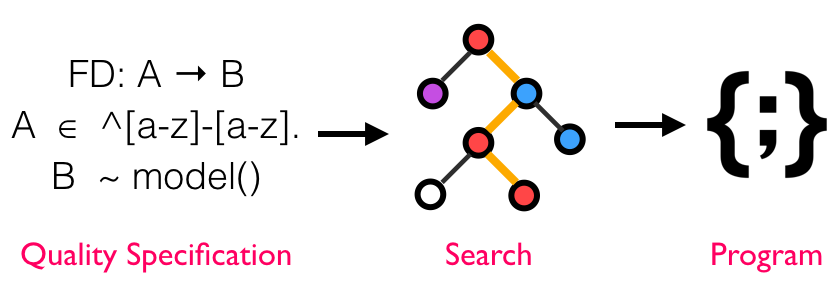
\includegraphics[width=\columnwidth]{figures/intro.png}
\caption{AlphaClean  is  given  a  specification  of  quality(e.g.,  integrity  constraints  or  a  statistical  model  the  data must conform to) and a language of allowed data transformations,  and it searches to find a sequence of transformations that best optimizes the quality specification.  }
\end{figure}

For example, one can represent cleaning with integrity constraints in this framework.
Consider a functional dependency relationship between zipcode and state $\textsf{Zip} \rightarrow \textsf{State}$. The quality function could be the number of tuples that satisfy the functional dependency.
The language of transformations is the set of functions that updates particular key pair $(z,s) \mapsto (z',s')$.
The search problem is to find a minimal sequence of such maps that optimizes the quality function.
The same framework can also handle numerical outliers.
Suppose, we have an anomaly detector that detects statistical outliers found in an aggregate view of the data.
We want to be able to find a filter on the base data that removes 
the outliers from the view.
The search problem is to find a minimal number of deletes that maximally removes outliers from the view.

This generality comes at the cost of the search time, and in general, this search problem is very difficult.
An efficient solution to this search problem would imply an efficient solution to all MAX-SAT instances.
Pragmatically, the system has to include optimizations that exploit the structure of typical data cleaning problems.
We specify these optimizations as pruning rules on the language of transformations.
These pruning rules can also be dynamic analyzing the quality functions and the data.
In fact, these pruning rules can also be learned where data can be cleaned in blocks or samples and operations that were unsuccessful in the past can be filtered.
This approach is inspired by similar approaches in AI, such as AlphaGo, which leverage learned scoring and pruning rules.
These optimizations can make this expensive search process more practical.

This approach has an additional benefit of applying to future unseen data.
By synthesizing a sequence of transformations, we are actually finding a program and not just a clean database instance.
This raises an important question not typically studied in the classical data integrity literature, namely, \emph{generalization}, where rules and transformations have to apply to future, unseen data.
Generalization in data cleaning is akin to generalization in machine learning, where simpler rules are likely to generalize and complex rules can overfit to the current database instance.
Implementing a form of ``regularization'' in this framework is straight-forward -- one simply has to restrict the language to less selective rules.



\subsection*{\sys}
We present \sys, a Python library that synthesizes data cleaning programs with search over a language of transformations.  
\sys is given a specification of quality (e.g., integrity constraints or a statistical model the data must conform to) and a language  of  allowed  data  transformations,  and  it  searches  to find a sequence of transformations that maximizes a quality metric derived from the specification.  

This paper presents several contributions:
\begin{enumerate}
\item We cast data cleaning as a search problem over a formal language of transformations to find a sequence of transformations that maximizes a quality metric, and present a system that implements this formalism with an API to specify pruning rules.
\item We describe how the search algorithm, which is a greedy best first search, can be parallelized, distributed, and can cache repeated computations.
\item We describe how pruning rules can be learned from previously cleaned data to improve performance.
\item The discovered  sequence of  transformations  defines  an  intermediate  representation,which can be easily transferred between languages or optimized with a compiler. We show how vectorization and loop fusion can be used to dramatically speed up the execution time of the data cleaning program.
\end{enumerate}
























\iffalse
While the search problem is exponential in the support of the language, we apply a number of novel optimizations including:  (1) hashing to remove search branches that lead to identical results, (2) merging branches that have non-conflicting  transformations,  and  (3)  leveraging  a best-first search algorithm called SSS*.

\begin{itemize}
  \item exsiting data cleaning/prep fit into a pattern that is a special case of optimization
  \item what information needed to represent each special case (goal, language etc)
  \item cleaning steps $>$ fixes
  \item iterating over languages $>$ specific lceaning steps
  \item HILDA === Cleaning
  \item show how it covers most elements of data cleanig/prep/analysis pipeline.  also includes things not well supported (numbers)
  \item benefits: pefr? HILDA, optimization framework, numerics, mix and match
  \item language integration with python makes it easy to define language
\end{itemize}

Then for the details

\begin{itemize}
  \item What is the model for readers to think about cleaning/prep etc?  Needed components?
  \item Distinguish objective function, running an operator and evaluating the result, and a cost estimate.
  \item How to think about pruning? beyond above bullet?  can optimizations from all other work fit into this framework easily?
  \item How does SGD fit in?  Is our stuff based on discrete optimization?  Branch and Bound?
  \item Greed best first tree search is only algorithm?  

\end{itemize}
\fi











